
\chapter{Terminology}
In all areas of research or vocation, there is terminology used that is specific to that field, and astronomy is no exception. Although this is not a treatise on the study of astronomy, it would serve you well to become acquainted with some of these terms.

\section{Disciplines of research}

You will hear terms such as \textit{astronomy, archaeoastronomy} and \textit{ethnoastronomy}. These terms can sometime become confusing so I will provide short definitions for them.

\subsection{Astronomy}
Astronomy is one of physical sciences and involves the systematic study of celestial objects and phenomena that originate outside the Earth's atmosphere. Astronomic data from various missions are recorded in catalogues for use within the scientific community. Within the field of study, there are various terms used, which are important to know in order to query and interpret the astronomical data you will encounter.

\subsubsection{Field of View}
The \textit{field of view} is the amount of sky that you are able to see and it is measured in degrees.  If we zoom in, we reduce the field of view. If we compare Figures~\ref{fig:fov60} and ~\ref{fig:fov13}, we see the same point of sky is in the centre, however, the image that looks closer has a lower field of view.

\begin{figure}[htbp]
	\centering
	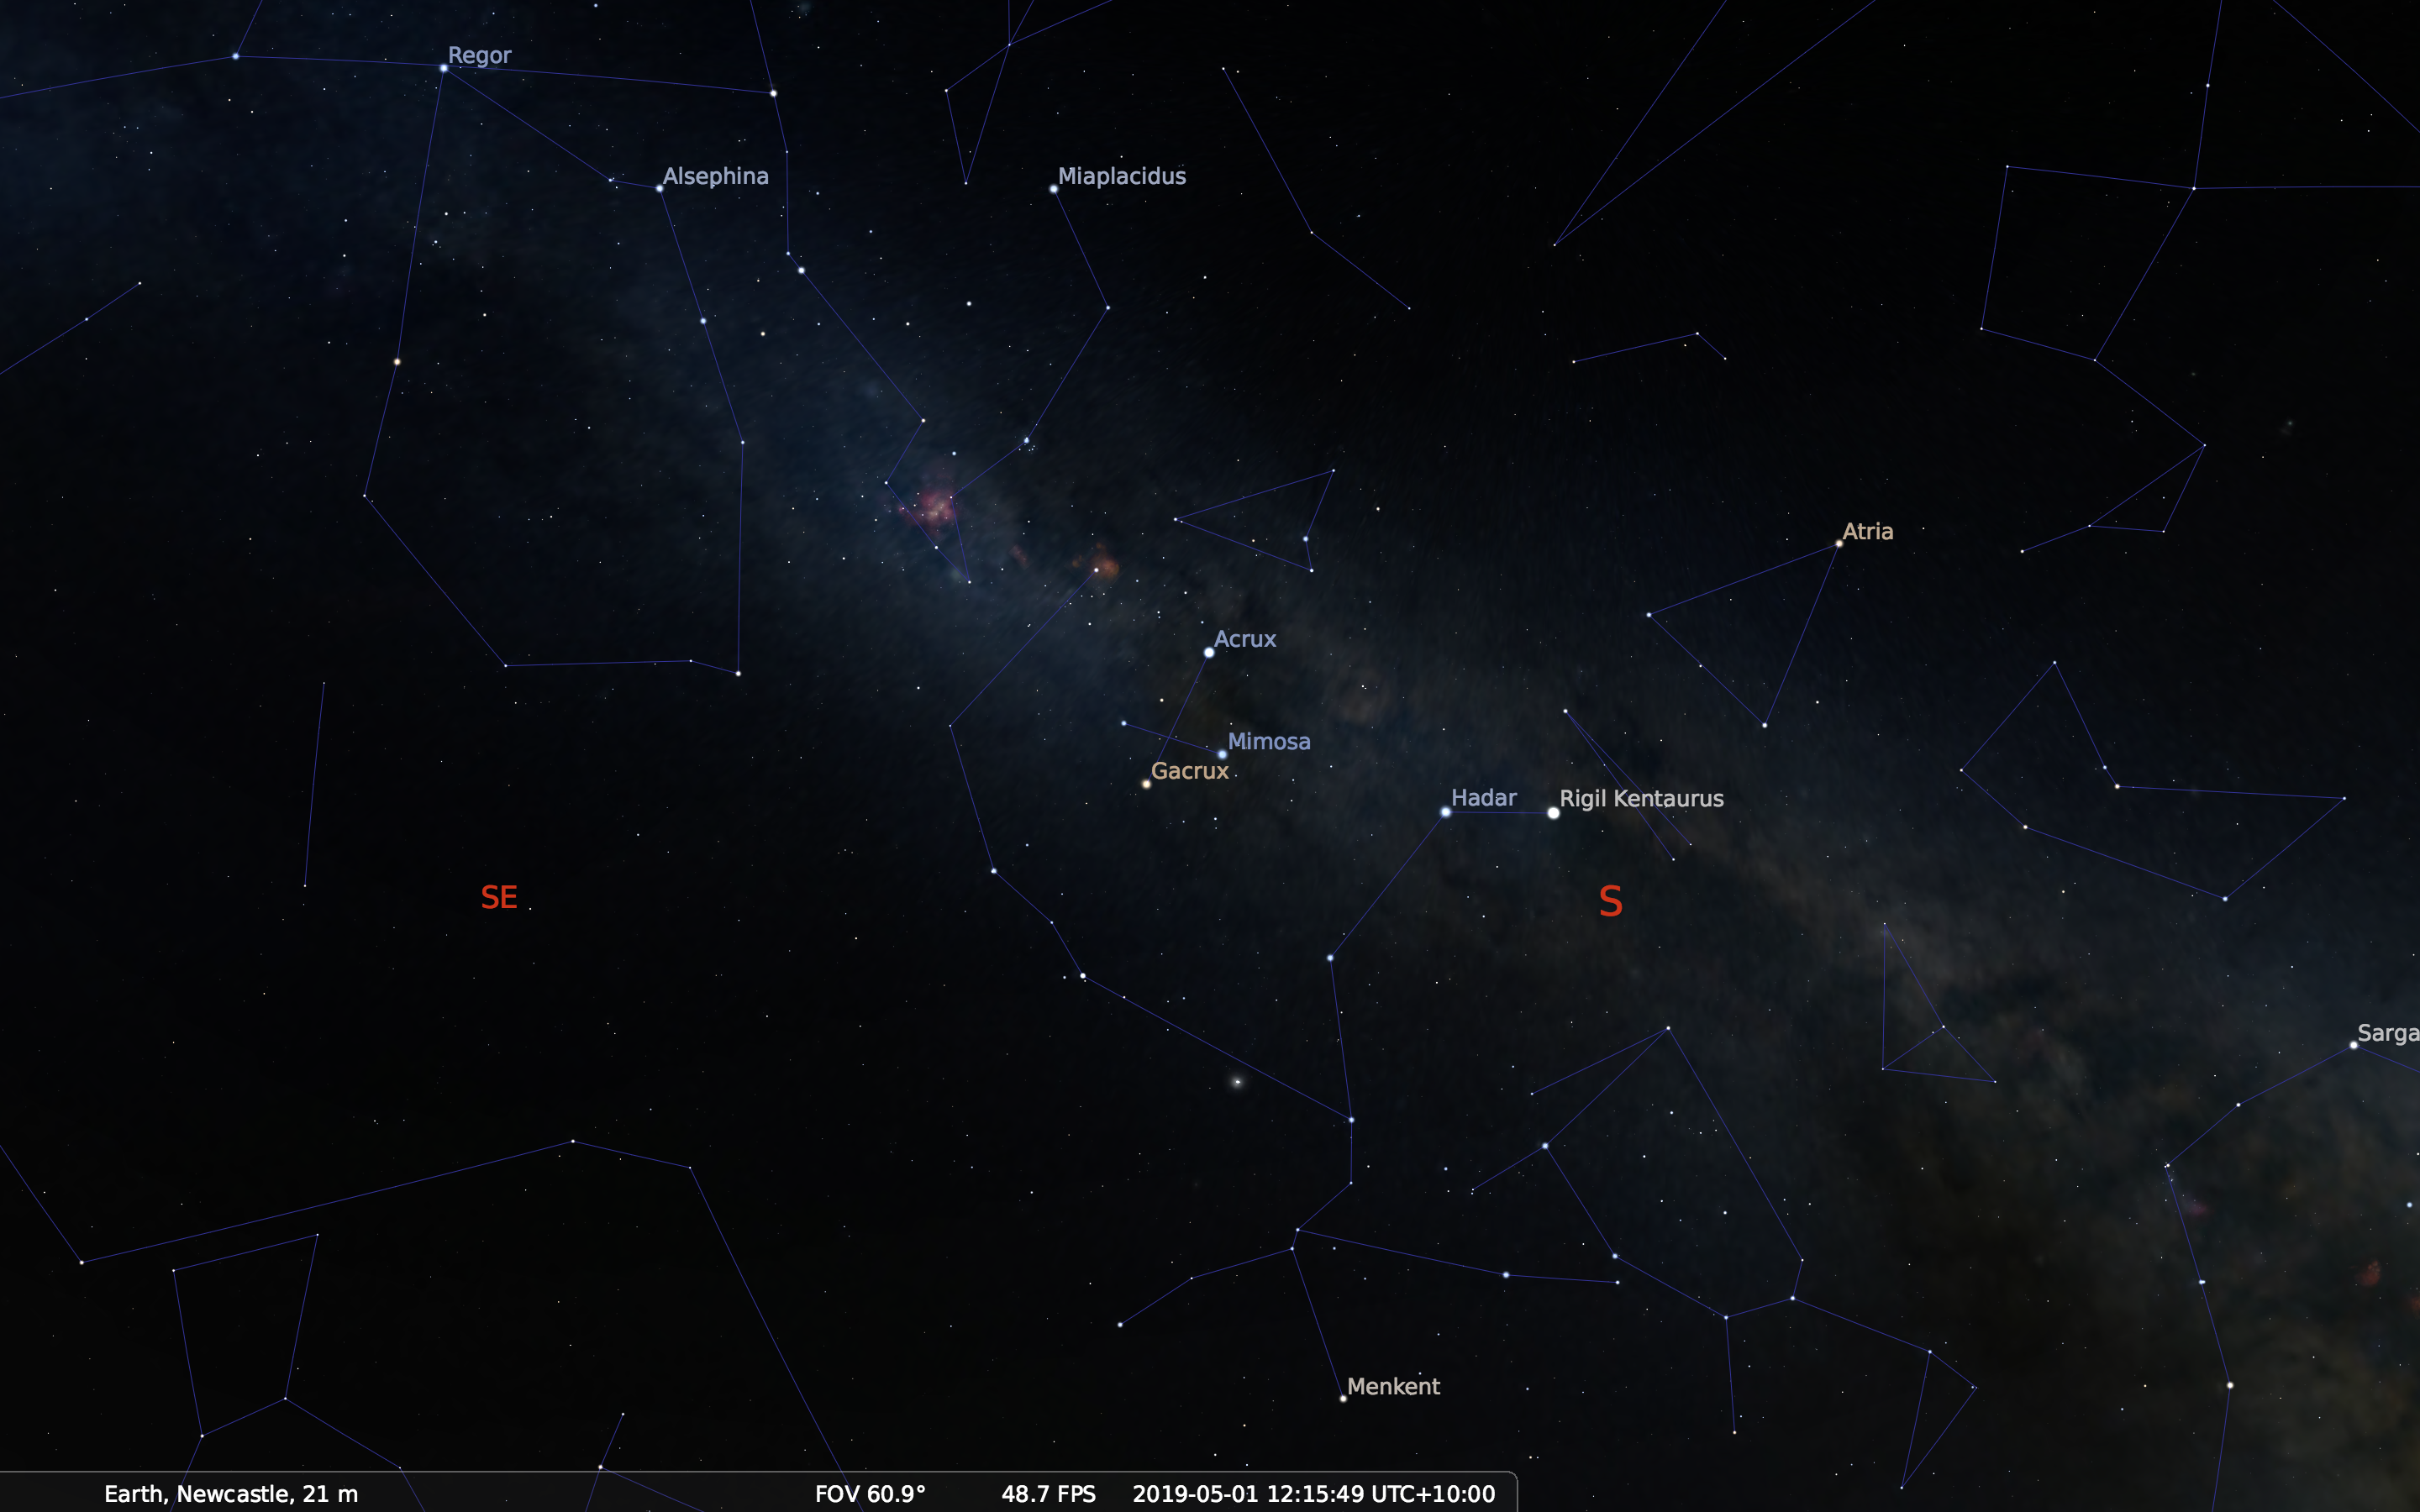
\includegraphics[width=0.5\columnwidth]{fov60}
	\caption{Stellarium displaying a 6060$^{\circ}$ field of view.}
	\label{fig:fov60}
\end{figure}

\begin{figure}[htbp]
	\centering
	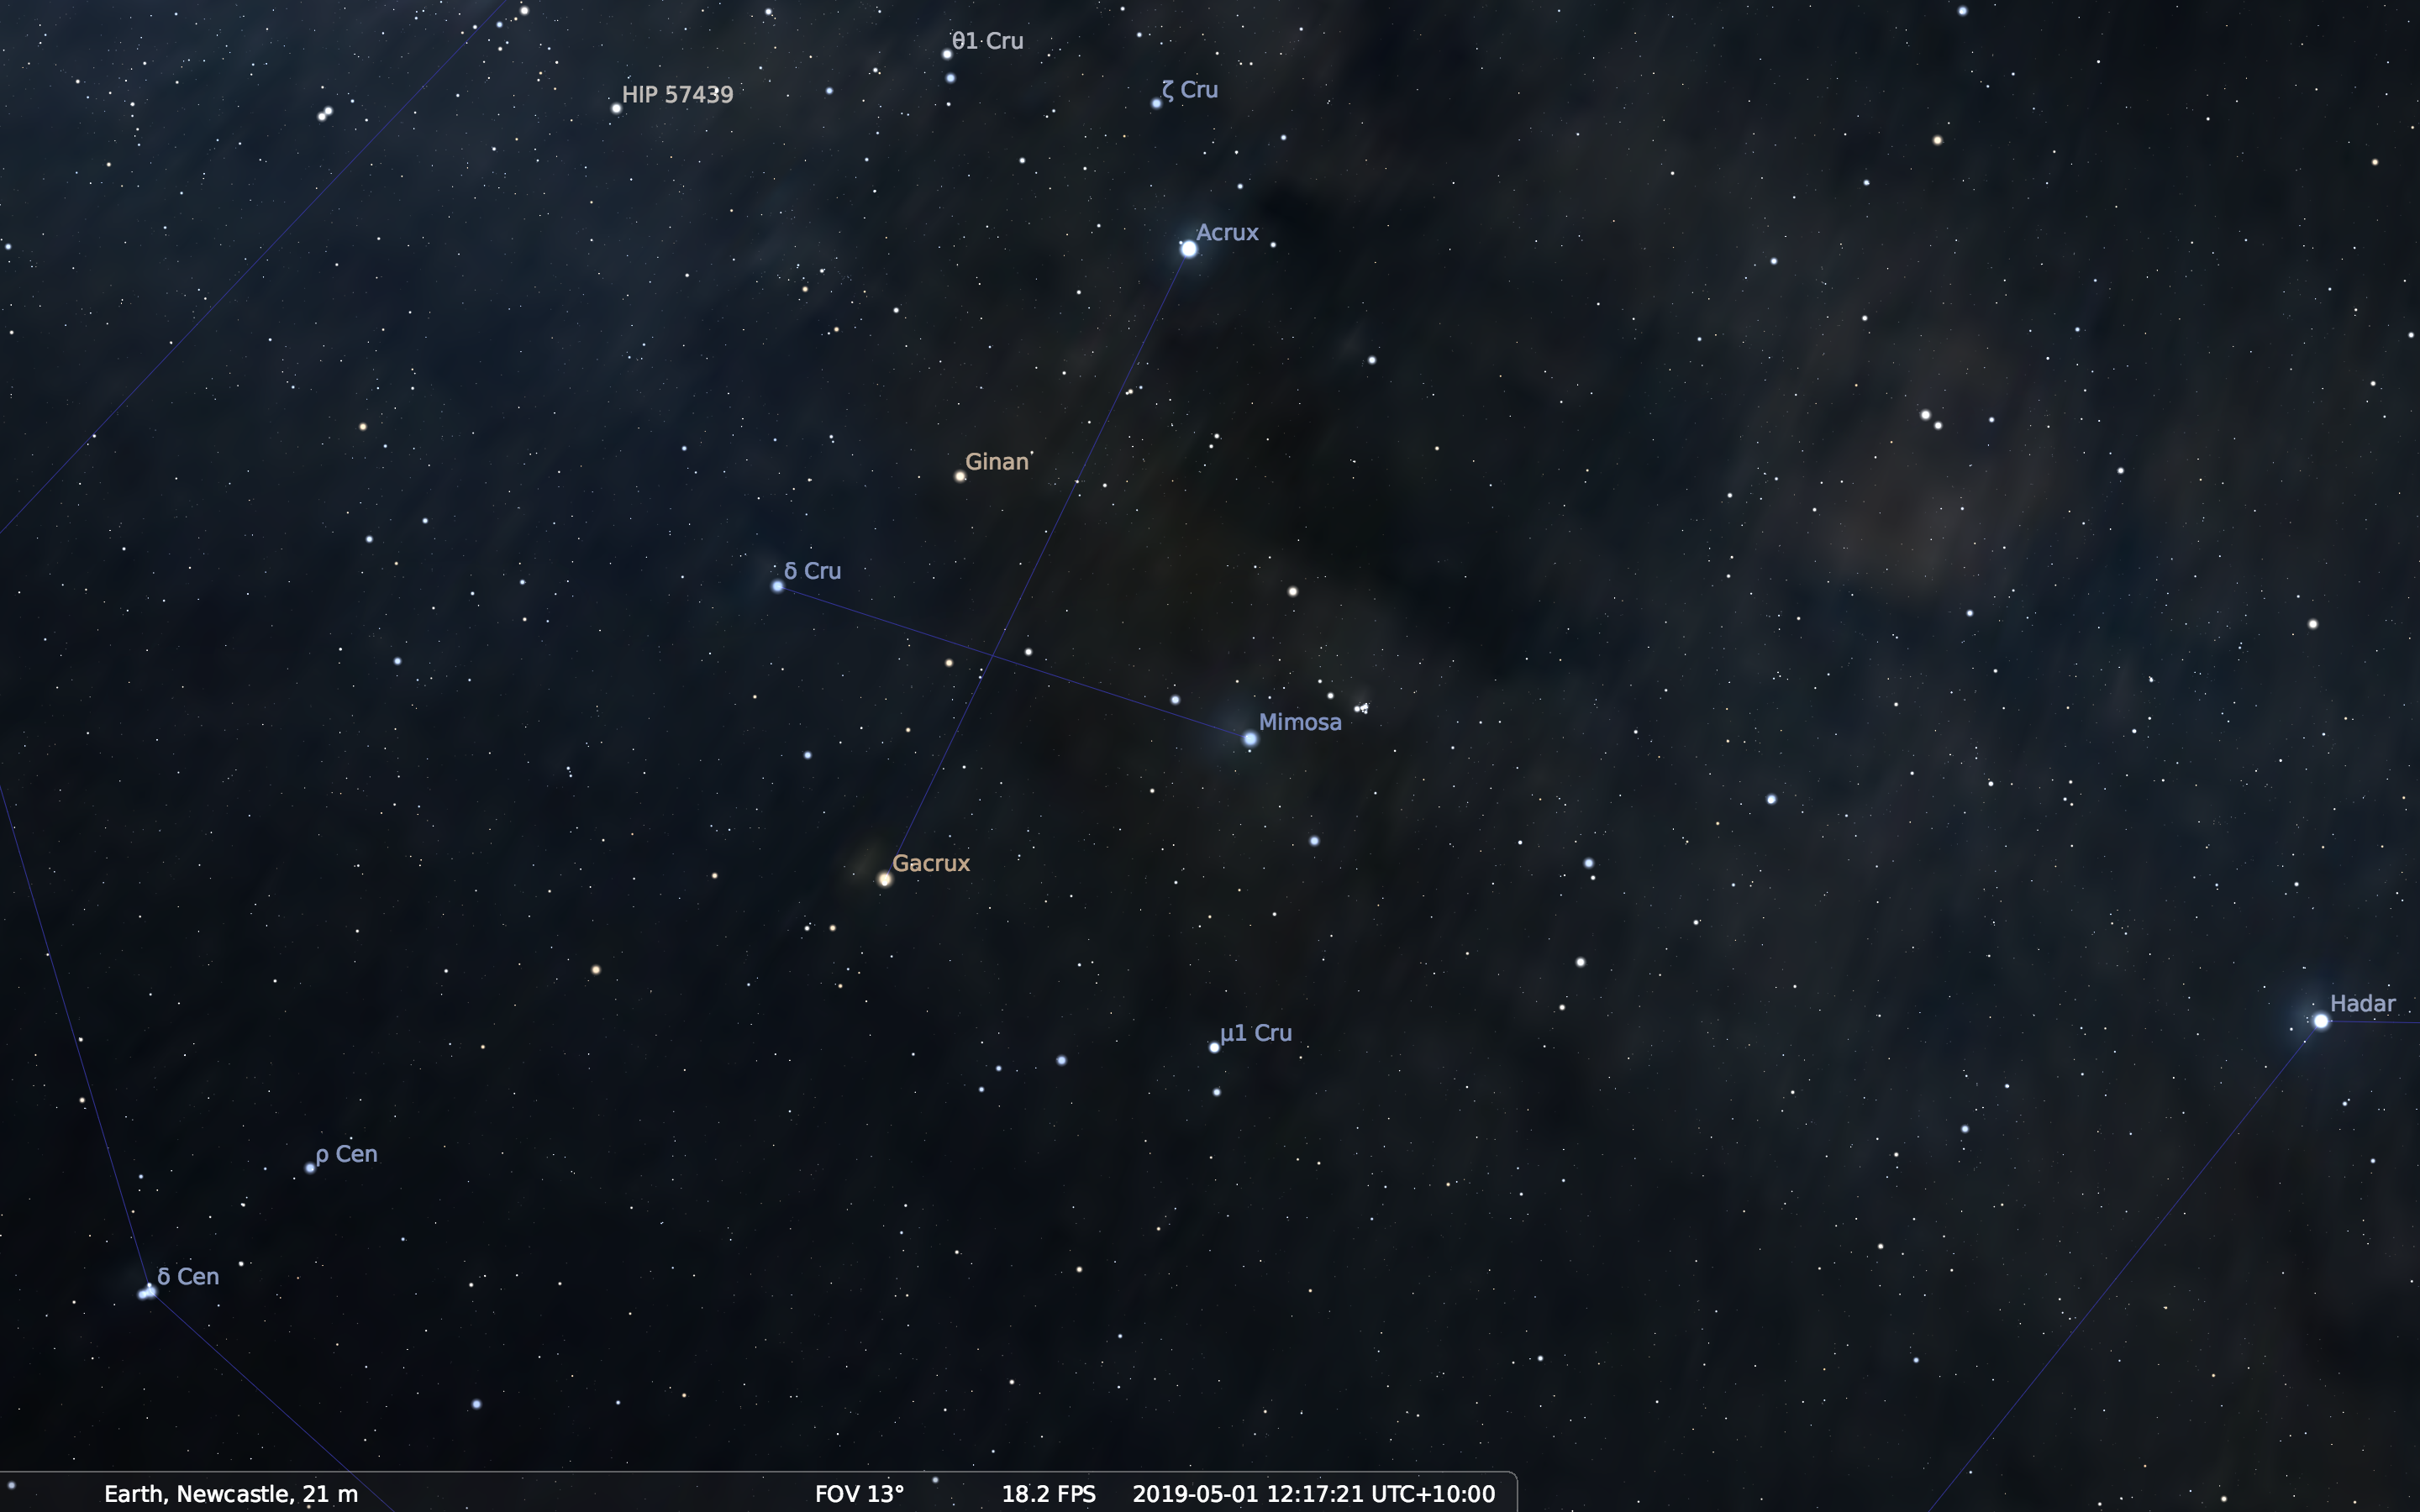
\includegraphics[width=0.5\columnwidth]{fov13}
	\caption{Stellarium displaying a 1360$^{\circ}$ field of view.}
	\label{fig:fov13}
\end{figure}

\subsubsection{Observation Location}

\subsubsection{Celestial Coordinates}
In the same way we can define an exact location on the Earth using latitude and longitude. For example, 32.9283$^{\circ}$ S, 151.7817$^{\circ}$  E
, we do the same with celestial objects using the celestial coordinate system
\subsubsection{Right Ascension}
The \textit{Right Ascension}, knows as the \textit{RA}, is the angular distance 

\subsubsection{Declination}


\subsubsection{Magnitude}

\subsubsection{Atmosphere}

\subsubsection{Mission}


\subsection{Ethnoastronomy}
Ethnoastronomy is a social science belonging to the discipline of ethnology and examines the way astronomy is practised in the context of a particular culture \cite{Salt2015}.

\subsection{Archaeoastronomy}
Archaeoastronomy is the study of how ancient civilisations understood the cosmos and in a sense very similar to ethnoastronomy.
``Broad public embrace of archaic astronomy probably began in the eighteenth
century with awareness of the summer solstice sunrise’s affiliation with Stonehenge" \cite[p.~263]{Krupp2015}.
Archaeoastronomers have used Stellarium to generate an astronomical display from a location for a period sometime in the past \cite{zotti2014towards}. 

\subsection{Astrology}
``Astrology, from the Greek, astro-logos, is the assumption that the stars and planets
contain meaning and significance for terrestrial affairs....Astrology appears to
be a universal feature of human culture and may be understood as a form of cultural
astronomy; an important contribution to the understanding of astronomy’s cultural
uses, applications, uses, and functions; and an indication of society’s attitudes to the
stars."\cite[p.~104]{Campion2015}.


	
